\documentclass[12pt]{zettel}

\usepackage{pdfpages}
\usepackage{booktabs}

\usepackage{geometry}
\geometry{tmargin=2cm,bmargin=4cm,lmargin=3.5cm,rmargin=3.5cm}

\renewcommand{\gregor}{\put(13.2,-3.0){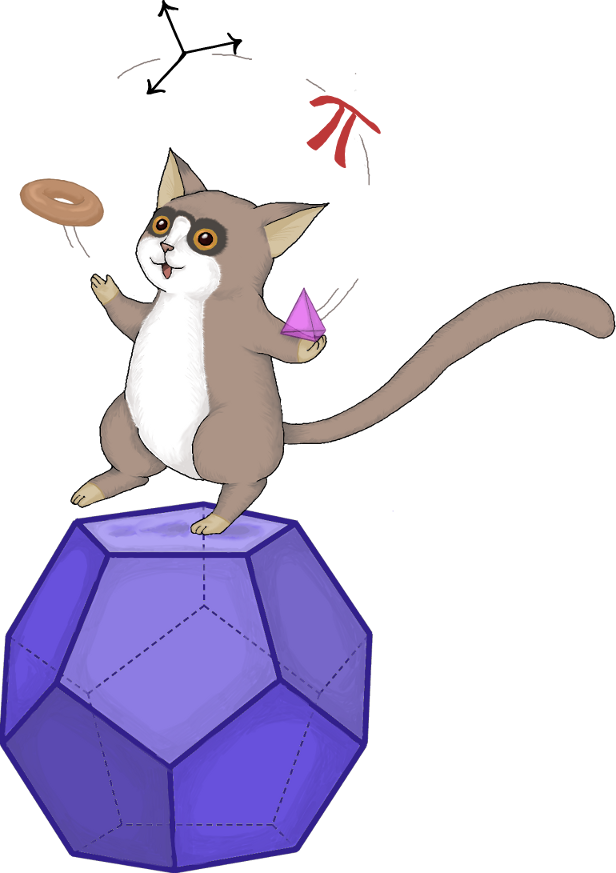
\includegraphics[scale=0.18]{cover}}}

\usepackage{framed}
\definecolor{shadecolor}{rgb}{.97,.97,.97}

\newcommand{\twopics}[2]{%
  \begin{figure}[b]%
    \vspace*{0.5cm}%
    \makebox[\textwidth][c]{%
      \includegraphics[width=0.6\textwidth]{impressionen/#1}%
      \hspace*{1cm}%
      \includegraphics[width=0.6\textwidth]{impressionen/#2}%
    }%
    \vspace*{-1cm}%
  \end{figure}
}

\begin{document}

\pagestyle{plain}

\renewcommand{\betreff}{}

\vspace{-2em}

\begin{center}
  {\qquad\quad}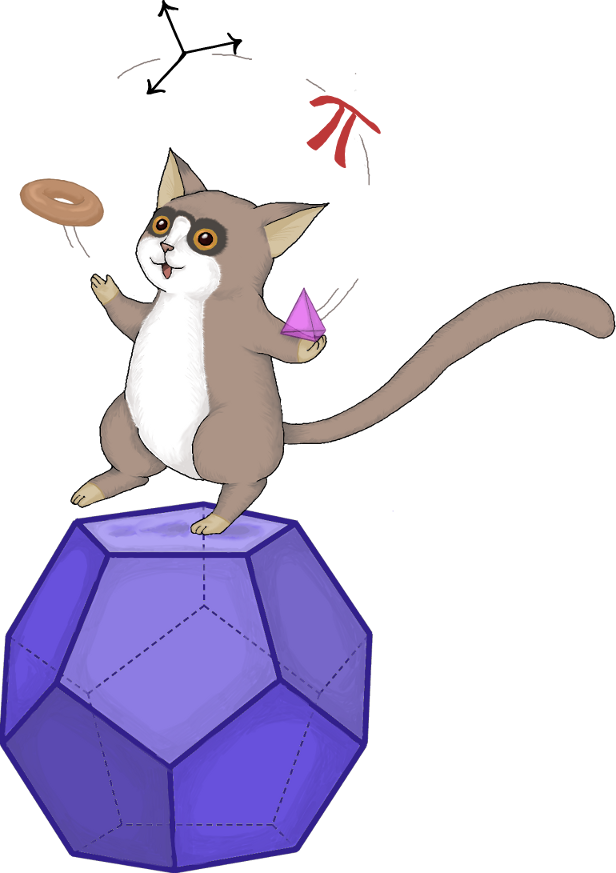
\includegraphics[scale=0.18]{cover}\\[1cm]

  \Large\textbf{\textsf{Das Mathecamp \\ des Matheschülerzirkels Augsburg}}
\end{center}

\vspace{1em}

Der Matheschülerzirkel Augsburg wurde im August~2013 zur Förderung des
Interesses und der Begeisterung für Mathematik unter Schülerinnen und Schülern
an weiterführenden Schulen jeglicher Schulart gegründet. Während des Schuljahrs~2013/2014 betreuten
19~Mitarbeiterinnen und Mitarbeiter ehrenamtlich die knapp
250~teilnehmenden Schülerinnen und Schüler in zweiwöchentlich an der
Universität stattfindenden Präsenzzirkeln. Für weiter entfernt wohnende Schülerinnen
und Schüler unterhielten wir monatliche Korrespondenz per Post. In den
Sommerferien 2014 veranstalteten wir mit 87~Teilnehmenden erstmalig ein fünftägiges Mathecamp.

Die Angebote des Matheschülerzirkels sind in Augsburg und Bayerisch-Schwaben einzigartig
und sollen langfristig weitergeführt und ausgebaut werden. Für das Mathecamp
2015 benötigen wir insgesamt etwa 10.000 \texteuro{} an finanziellen
Zuschüssen.

Zum Zwecke der besseren Lesbarkeit wird im Folgenden das generische Femininum verwendet. Soweit nicht jeweils anders erklärt, sind damit natürlich immer Personen jeglichen
Geschlechts gemeint.

\thispagestyle{empty}
\enlargethispage{4em}
\vspace{-2em}
\renewcommand\contentsname{}
\tableofcontents


\section{Unsere Vision}

Das Ziel des Matheschülerzirkels ist es, Schülerinnen langfristig eine Möglichkeit zu bieten, ihrem Interesse an der
Mathematik über den Unterricht hinaus nachzugehen. Wir möchten Kinder, die Spaß an der Mathematik gefunden haben, dazu animieren und darin unterstützen, sich weiter
mit der Mathematik zu beschäftigen. Es geht uns darum, diesen Schülerinnen zu zeigen, wie spannend Mathematik sein kann und wie diese außerhalb der Schule aussieht.

Im Gegensatz zu anderen Hobbys wie beispielsweise Sport und Musik gibt es für die Mathematik kaum Angebote außerhalb des Schulunterrichts, die nicht der Nachhilfe dienen.
In der Grundschule haben viele Schülerinnen noch eine ausgeprägte Begeisterung für 
Rätsel und mathematische Spiele, die leider oft im Laufe der weiteren
Schulzeit verloren geht. Diese Begeisterung möchten wir
durch unser Angebot erhalten und sogar noch ausbauen, indem wir
unseren Teilnehmerinnen ermöglichen, sich frei von jeglichem
(Noten-)Druck mathematische Themen zu erarbeiten.

\twopics{auftakt1}{auftakt2}

Ein wichtiger Aspekt ist dabei die Vernetzung Gleichgesinnter. Durch unsere Angebote können interessierte
Schülerinnen ihrem Hobby Mathematik gemeinsam in einem motivierenden Umfeld nachgehen. Viele der Mitwirkenden haben selbst als Schülerinnen von derartigen Angeboten
profitiert und können aus eigener Erfahrung hervorheben, wie wichtig die so gewonnenen Freundschaften und Erlebnisse für die persönliche Entwicklung sein können.

Der Wesen der Mathematik ist die logische Untersuchung von abstrakten Strukturen. Im Vordergrund steht dabei nicht das Auswendiglernen und Anwenden von Lehrsätzen, sondern
das Hinterfragen und Verstehen, warum ein Lehrsatz denn wahr ist. Die Beschäftigung mit Mathematik schult also das analytische Denken und das methodische Vorgehen beim Lösen
von Problemen. Deshalb macht die Teilnahme am Matheschülerzirkel nicht nur Spaß und Freude, sondern hilft den Teilnehmerinnen auch dabei, kritisches Denken
zu entwickeln und zu selbstständigen Persönlichkeiten heranzuwachsen.

\newpage

Es ist zu befürchten, dass einige an Mathematik interessierte Schülerinnen mit dem sich immer noch haltenden, aber unsinnigen Vorurteil, dass "`Mathe nichts für Mädchen sei"',
konfrontiert werden. Während am Ende der Grundschulzeit das Interesse am Rechnen und an Rätseln bei beiden Geschlechtern in etwa gleich verbreitet ist, scheint dieses mit
dem Älterwerden bei Mädchen stärker zu schwinden. Es ist zu vermuten, dass dabei die geschlechtsspezifischen Stereotype, die das soziale Umfeld leider zu oft vermittelt, einen
erheblichen Einfluss haben.

Ein wichtiges Ziel des Matheschülerzirkels ist es, diesen Vorurteilen entgegen zu wirken. Um zu verhindern, dass Eltern wegen der Skepsis, ob denn ihre
Tochter wirklich für "`so schwierige Mathematik"' geeignet sei, von einer Anmeldung absehen, achten wir selbstverständlich bei der Formulierung und dem Design von Aushängen und Flyern
darauf, uns keiner Stereotypen zu bedienen.

Weiterhin ist unser gesamtes Angebot niedrigschwellig gestaltet, nicht zuletzt deswegen, um nicht ebenjene skeptischen Eltern
von der Anmeldung abzuhalten. Außerdem bitten wir alle Fachbetreuerinnen der Schulen in Bayerisch-Schwaben, die wir über unseren Zirkel informieren, interessierte weibliche Schülerinnen an
einer Teilnahme zu ermutigen. Für junge Schülerinnen etablieren wir weibliche Zirkelleiterinnen als Vorbilder, und nicht zuletzt sind die von uns erstellten Aufgaben stets so formuliert, dass keine Genderstereotypen reproduziert werden. Natürlich sind sämtliche Betreuerinnen des
Matheschülerzirkels für diese Thematik sensibilisiert.

Es freut uns sehr, dass im vergangenen Schuljahr
40~Prozent der Teilnehmenden an Präsenz- und Korrespondenzzirkeln weiblich waren. In den Klassenstufen~5 und~6 war die Quote sogar ausgeglichen. Wir möchten in Zukunft insbesondere
in den höheren Jahrgangsstufen noch mehr Mädchen für den Mathezirkel begeistern.

\twopics{klein-04}{klein-08}


\section{Über uns}

Der Matheschülerzirkel Augsburg ist eine Einrichtung des
Mathematisch-Phy\-si\-ka\-li\-schen Vereins e.\,V. und wird organisiert von
Mitarbeiterinnen der Universität
Augsburg. Er setzt sich aus Doktorandinnen
und engagierten Studentinnen zusammen.

Begonnen wurde das Projekt als informeller Zusammenschluss von motivierten Doktorandinnen. Da ein Ziel des Mathematisch-Physikalischen Vereins~e.\,V. in Augsburg die Darstellung
der Mathematik in der Öffentlichkeit ist, fanden sich gemeinsame Interessen, und der Matheschülerzirkel ist nun im Rahmen des~Vereins organisiert.

Die Professorinnen des Instituts für Mathematik unterstützen den
Mathe\-schü\-ler\-zir\-kel nach Kräften, er ist aber keine Einrichtung der Universität
Augsburg, sondern wird eigenständig und eigenverantwortlich von den beteiligten Studierenden und Doktorandinnen organisiert.

Ein Großteil der Mitwirkenden hat bereits langjährige Erfahrung in
der Jugendarbeit und in der Mathematikbildung. Viele von uns nahmen früher selbst an Mathematikzirkeln oder
Mathecamps in anderen Regionen teil und möchten nun ihre eigenen prägenden Erfahrungen an die Schülerinnen Augsburgs und Bayerisch-Schwabens weitergeben.

\begin{center}\small
\renewcommand{\arraystretch}{1.13}
\begin{tabular}{@{}p{4.0cm}@{\qquad}p{6cm}@{\qquad}l@{}}
  \toprule
  \multicolumn{3}{@{}l@{}}{\textbf{Zirkelleiterinnen}} \\
  \toprule
  \textbf{Name} & \textbf{Akademischer Grad} & \textbf{Alter} \\
  Meru Alagalingam & Diplom in Mathematik & 23 \\
  Tim Baumann &  & 20 \\
  Martin Baur & B.\,Sc.\ in Mathematik & 26 \\
  Ingo Blechschmidt & M.\,Sc.\ in Mathematik & 26 \\
  Tim Dafler & & 21 \\
  Dominik Dirr & Staatsexamen Mathematik (Gymn.) & 25 \\
  Philipp Düren & M.\,Sc.\ in Mathematik & 23 \\ 
  Alexander Engel & M.\,Sc. in Mathematik & 27 \\ 
  Johanna Fleckenstein & M.\,Sc.\ in Mathematik & 26 \\ 
  Lukas Graf & & 23 \\
  Anne Grünzig & Diplom in Mathematik & 33 \\
  Kathrin Helmsauer & M.\,Sc.\ in Mathematik & 24 \\ 
  Christian Hübschmann & Diplom in Mathematik & 29 \\ 
  Jil Hümmer & Staatsexamen Mathematik (Gymn.) & 25 \\
  Simon Kapfer & M.\,Sc.\ in Mathematik & 26 \\ 
  Sven Prüfer & M.\,Sc.\ in mathematischer Physik & 27 \\ 
  Lisa Reischmann & M.\,Sc.\ in Mathematik & 27 \\
  Caren Schinko & Staatsexamen Mathematik (Gymn.) & 24 \\
  Johannes Sedlmeir & & 22 \\
  Benedikt von Seelstrang & B.\,Sc. in Mathematik & 23 \\
  Peter Uebele & M.\,Sc.\ in mathematischer Physik & 25 \\ 
  Carina Willbold & M.\,Sc.\ in Mathematik & 26 \\ 
  Stephanie Zapf & M.\,Sc.\ in Mathematik & 27 \\
\bottomrule
\end{tabular}
\end{center}

\newpage

Der Matheschülerzirkel Augsburg besteht neben dem Mathecamp aus mehreren einander ergänzenden Veranstaltungen, die im
Folgenden einzeln beschrieben werden. Interessierte Schülerinnen
können diese unabhängig voneinander besuchen. Bis auf das Mathecamp sind alle
Veranstaltungen für die Teilnehmenden kostenlos. Einzige
Teilnahmevoraussetzungen sind Spaß und Interesse an der Mathematik. Es gibt
insbesondere keine Teilnahmebeschränkung durch Noten, Schulzugehörigkeit oder
Wettbewerbsergebnisse.

In Bayrisch-Schwaben gibt es vereinzelte, deutlich kleinere lokale
Projekte, die ähnlich wie das unsere auf Mathematikförderung bei Schülerinnen ausgerichtet sind. Diese sind aber entweder nur an einzelnen Schulen
angesiedelt und stehen daher nur wenigen Jugendlichen zur Verfügung, oder zielen
auf Mathematiknachhilfe ab. Der Matheschülerzirkel Augsburg ist das erste
Projekt in Bayerisch-Schwaben, das unabhängig von schulischen Leistungen und der besuchten Schulart die
Begeisterung für Mathematik fördern und erhalten möchte.

Es grenzt sich deutlich von Nachhilfeangeboten ab, da wir Themen behandeln, die in keiner Schulart auf dem Lehrplan stehen. Somit werden Unterrichtsinhalte weder
vorweggenommen noch wiederholt und es handelt sich nicht um Nachhilfe.

An anderen Orten wie Leipzig\footnote{\href{http://lsgm.uni-leipzig.de/tiki-index.php}{\textsf{http:/\!/lsgm.uni-leipzig.de/tiki-index.php}}} und
Stuttgart\footnote{\href{http://www.mathematik.uni-stuttgart.de/studium/schuelerzirkel/}{\textsf{http:/\!/www.mathematik.uni-stuttgart.de/studium/schuelerzirkel/}}}
werden ähnliche Projekte seit
vielen Jahren mit 150 bis 200 Teilnehmenden erfolgreich durchgeführt. Der überwältigende Ansturm auf die Präsenz- und Korrespondenzzirkel des vergangenen Schuljahrs sowie auf das
erste Mathecamp zeigte, dass auch hier in Augsburg und Umgebung Nachfrage und großes Interesse besteht.

Um auf die Initiierung unseres Projekts zu Beginn des Schuljahrs~2013/2014
aufmerksam zu machen, schickten wir allen Gymnasien Schwabens und einigen
weiteren Schulen im Umkreis von Augsburg Informationspakete mit Lehrerinnenbriefen,
Flyern und Plakaten. Um sicherzugehen, dass unser Angebot in der
Vielzahl der Korrespondenz bei den Schulen nicht unterging, befragten wir außerdem
die Studenten der Universität nach Lehrerinnen, die zu ihrer Schulzeit
besonders großes Engagement gezeigt hatten, und schrieben diese separat an.
Häufig zeigten sich diese sehr angetan von unserem Projekt.

Weiterhin griff die Lokalpresse, insbesondere die regionale Tageszeitung
\emph{Augsburger Allgemeine}, unsere Pressemitteilung auf und bereitete sie zu einem prominenten Artikel auf (siehe Anlage). Weitere mediale Präsenz erhielten wir durch das Augsburger
Regionalfernsehen \emph{a.tv}, das eine kurze Reportage über den Matheschülerzirkel drehte.\footnote{\href{http://www.augsburg.tv/aktuell/schuelerzirkel-mathematik-30_12_2013.html}{\textsf{http:/\!/www.augsburg.tv/aktuell/schuelerzirkel-mathematik-30\_{}12\_{}2013.html}}} Auf diese Weise konnten wir insgesamt etwa~250 Schülerinnen für
unser Projekt begeistern, davon~120 aus dem Großraum Augsburg.

Der Großteil unserer Teilnehmerinnen besucht Gymnasien, es machen aber auch einige Realschülerinnen mit. Auch Fachoberschülerinnen steht unser Angebot offen, in diesem Jahr werden wir dort verstärkt werben.

Etwa zwei Drittel unserer Teilnehmenden
stammen aus den Klassenstufen~5 bis~8.
Dies deckt sich mit der
Erfahrung an anderen Orten, dass anfangs ein größeres Interesse für
Mathematik besteht und dieses oft im Laufe der Pubertät
deutlich nachlässt -- ein Problem, dem wir gezielt begegnen. Unser Ziel ist, die Schülerinnen über ihre gesamte Schullaufbahn hinweg zu begleiten.

In den Korrespondenzzirkeln betreuen wir Schülerinnen aus ganz Bayerisch-Schwaben, sowie vereinzelt darüber hinaus. Dagegen kommen die Teilnehmerinnen
der Prä\-senz\-zir\-kel alle aus dem Großraum Augsburg. Viele von ihnen
nehmen an beiden Zirkeln teil.


\section{Angebote während des Schuljahrs}

\subsection{Präsenzzirkel}

Die Präsenzzirkel finden in nach Klassenstufe eingeteilten
Kleingruppen von fünf bis zehn Schülerinnen statt.
Die jeweilige Gruppe trifft sich nachmittags alle zwei Wochen mit ihrer Zirkelleiterin auf dem Campus der Universität Augsburg und diskutiert und
bearbeitet in gut 90~Minuten Themen der Mathematik, die außerhalb des
Schulstoffs liegen. Durch die kleine Gruppengröße können wir individuell auf
Vorkenntnisse und Themenwünsche eingehen.

Der Ablauf eines Präsenzzirkels hängt stark von der Klassenstufe ab. Bei den
jüngeren Kindern werden Themen eher durch Bearbeiten von passenden
Aufgaben in Eigeninitiative erkundet, während Schülerinnen höherer
Klassenstufen auch durch geleitete Diskussionen in der Gruppe
Themen erarbeiten können. In vielen Zirkeln finden spezielle Materialien,
wie zum Beispiel Zauberwürfel, selbstgeschriebene Computerprogramme oder
Bastelutensilien Verwendung.

Eine Leistungskontrolle der Teilnehmerinnen spielt dabei keine Rolle. Uns ist es wichtig, dass sich alle Teilnehmerinnen frei von Konkurrenzdruck mit für sie interessanten
und angemessenen Themen beschäftigen können. Durch eine große Auswahl an vorbereiteten Aufgaben und Rätseln zum aktuellen Thema können die Zirkelleiterinnen dabei für
jede Teilnehmerin individuell passende Angebote präsentieren, sodass alle den Erfolg selbst erarbeiteter Lösungen genießen können.

Die Themen sind sehr vielfältig und reichen unter anderem von
Knobelaufgaben, geheimen Botschaften, Fibonacci-Zahlen und Nim-Spielen (ab Klasse 5),
über Zahlentheorie, Geometrie, Programmierung und Zauberwürfeln (ab Klasse 7) bis hin zu
Fraktalen und Chaos, vierdimensionaler Geometrie und nichtklassischer Logik
(ab Klasse 9). Zusätzlich bieten wir einen Zirkel an, der inhaltlich stärker an
mathematischen Wettbewerben ausgerichtet ist.

Die Präsenzzirkel bieten den Teilnehmerinnen die Möglichkeit,
gemeinsam mit weiteren mathematisch interessierten Jugendlichen außerhalb der
Schule Mathematik zu betreiben. Sie sind für die Schülerinnen kostenlos und der Einstieg ist jederzeit möglich. Im vergangenen Schuljahr konnten wir insgesamt zehn
Präsenzzirkelgruppen einrichten.

\subsection{Korrespondenzzirkel}

Viele unserer Schülerinnen können aus verschiedenen Gründen
nicht zu unseren Prä\-senz\-zir\-keln kommen, in erster Linie, weil sie zu weit
entfernt von Augsburg wohnen oder zu viele andere Termine haben.
Daher bieten wir auch schriftliche Korrespondenzzirkel per Post
an.

Wie die Präsenzzirkel sind die Korrespondenzzirkel nach Klassenstufen eingeteilt. Ein
Korrespondenzbrief enthält ein von der Zirkelleiterin geschriebenes Skript zu einem mathematischen Thema sowie passende
Übungsaufgaben. Teilweise bauen dabei die Themen aufeinander auf, sodass in den Korrespondenzzirkeln über mehrere Briefe hinweg umfangreiche oder komplexere Themen erarbeitet
werden können. Die Jugendlichen haben pro Brief etwa vier Wochen Zeit, um sich
mit der Materie auseinanderzusetzen, die Aufgaben zu bearbeiten und ihre Ergebnisse
an uns zu schicken. Die Zirkelleiterinnen senden dann
ausführliche Korrekturen und Tipps zurück.

Dabei spielen der Umfang oder die Qualität der abgegebenen Lösungen eine untergeordnete Rolle, wir freuen uns über jede Beschäftigung
mit den angebotenen Themen und möchten diese Wertschätzung auch den Teilnehmerinnen übermitteln. Die Korrektur der Aufgaben dient nicht dem Leistungsvergleich mit anderen
Teilnehmerinnen, sondern soll die individuellen Stärken hervorheben und bei Problemen Hilfestellung geben, diese in Zukunft zu vermeiden.

Thematisch ähneln sich die beiden Zirkelarten. Wie bei den
Präsenzzirkeln ist die Teilnahme kostenlos, der Einstieg ist zu Beginn jedes Themenblocks möglich.


\subsection{Mathematikolympiade}

Im Februar 2015 werden wir auf dem Campus der Universität die Landesrunde der Mathematikolympiade für Schülerinnen der Klassenstufen~5 und~6 aus dem Großraum
Augsburg durchführen. Die Mathematikolympiade ist ein internationaler Klausurwettbewerb, dessen mehrstufige Auswahlklausuren für die Bundesrunde
bislang dezentral an den einzelnen Schulen durchgeführt wurden. Seit einigen
Jahren gibt es zentrale Landesrunden für die Klassenstufen~7 und höher, die von
\emph{Mathematik-Olympiade in Bayern e.\,V.} organisiert werden.

Da es aber insbesondere für Schülerinnen aus den Klassenstufen~5
und~6 etwas ganz Besonderes ist, für ihre Erfolge in der zweiten Stufe
eingeladen zu werden und die Klausur der Landesrunde gemeinsam mit anderen
Teilnehmerinnen zu schreiben, möchten wir diese Veranstaltung
ins Leben rufen.

Dazu laden wir im Februar 2015 ungefähr~50 der in der zweiten Stufe
erfolgreichsten Fünft- und Sechstklässlerinnen des Großraums
Augsburg zu uns ein. Diese schreiben dann gemeinsam ihre Olympiadeklausur und
können sich am Nachmittag während der Korrektur unter Betreuung kennenlernen
und austauschen. Abschließend gibt es eine offizielle Siegerehrung.

Eine zentrale Landesrunde ist eine gute Möglichkeit, die sonst von
Hausaufgabenwettbewerben geprägte Mathematikwettbewerbslandschaft durch
Klausurwettbewerbe zu erweitern und dadurch mathematikbegeisterte Schülerinnen
zusammenzuführen. Solche für die Schülerinnen
sehr besonderen Erfahrungen steigern auch ihr Selbstwertgefühl. Sie zeigen
den Jugendlichen, dass ihre Begeisterung für Mathematik geschätzt wird und dass sie eigenständig Ziele erreichen können.

Wir hoffen, dass sich dadurch auch die Teilnehmerinnenzahl an der Olympiade
in den höheren Klassenstufen langfristig erhöht.


\subsection{Weitere Aktivitäten}

Neben den bereits genannten Zirkeln, dem Mathecamp und der
Matheolympiade organisieren wir noch weitere kleinere
Aktivitäten.

Die wichtigsten zwei Veranstaltungen dieser Art sind die Auftakt- sowie die
Abschlussveranstaltung. Am 9. November 2013 fand unsere erste
Auftaktveranstaltung mit einem anschaulichen und für alle Klassenstufen
geeigneten Vortrag von
Prof.~Dr.~Jost-Hinrich Eschenburg zum Thema \emph{Was sind eigentlich die
Zahlen?} statt, bei der wir auch die Termine für die Präsenzzirkel absprachen.
Die über 150 Teilnehmerinnen und ihre Eltern waren durchweg
begeistert.

Am Ende des Schuljahrs gab es eine Abschlussveranstaltung mit einem
weiteren mathematischen Vortrag, bei der wir
das vergangene Jahr in den Zirkeln Revue passieren ließen und als Anerkennung
Preise verliehen und mathematische Kleingeschenke verteilten. Diese beiden Veranstaltungen sollen
auch in den kommenden Jahren dem Zirkelschuljahr einen Rahmen geben.

Des Weiteren besuchen wir mit unseren Präsenzzirkelteilnehmenden die
Vortragsreihe \emph{Faszination Mathematik und Physik}, in welcher viermal im
Jahr Augsburger Professorinnen der Mathematik und Physik ihre Forschung der
Öffent\-lich\-keit anschaulich darlegen. Außerdem unterstützen wir
Mathematik betreffende Aktionen wie den \emph{Tag der Mathematik} an
der Universität Augsburg oder den \emph{Girls' Day}.

Im kommenden Schuljahr möchten wir Wochenendtreffen für die Teil\-neh\-mer\-in\-nen der Korrespondenzzirkel anbieten, um auch diesen Jugendlichen die
Möglichkeit zu bieten, sich mit Gleichgesinnten auszutauschen. Diese Treffen
sollen etwa zweimal pro Jahr stattfinden.

Außerdem möchten wir an mehreren Wochenenden einzelne Vorträge in einem
größeren Rahmen anbieten, vorrangig für Schülerinnen aus Augsburg.
Die Vorträge sollen von auswärtigen Mathematikerinnen aus Wirtschaft und Wissenschaft gehalten werden.


\newpage

\subsection{Finanzierung}

Im Vergleich zum Mathecamp verursachen uns die meisten unserer Angebote nur
geringe Kosten. Diese deckten wir im Schuljahr~2013/2014 durch eine interne
Spende des Mathematisch-Physikalischen Vereins (500 \texteuro), durch eine
Zuwendung vom \emph{Bündnis für Augsburg} (Maximalförderbetrag, 500~\texteuro),
einer Einrichtung der Stadt Augsburg,
sowie durch einmalig verfügbare MINT-Mittel (1000 \texteuro). Für
das Schuljahr~2014/2015 haben wir bislang keine Fördermittel.

\bigskip
\bigskip

\makebox[\textwidth][c]{%
  \small%
  \renewcommand{\arraystretch}{1.2}
  \begin{tabular}{@{}p{4.4cm}@{\qquad}r@{\qquad}p{7.2cm}@{}}
    \toprule
    \multicolumn{3}{@{}l@{}}{\textbf{Jahresbudget pro Schuljahr}} \\
    \toprule
    Auftaktveranstaltung & 500 \texteuro & Verpflegung, Flyer, Plakate \\
    Zirkelmaterialien & 1.000 \texteuro & Bücher zur Kursvorbereitung, Bastel- und Anschauungsmaterialien \\
    Korrespondenzzirkeltreffen & 2 \texttimes{} 300 \texteuro & ab 2015 \\
    Vortragssamstage & 2 \texttimes{} 300 \texteuro & ab 2015 \\
    Mathematikolympiade & 1.500 \texteuro & ab 2015 \\
    Abschlussveranstaltung & 700 \texteuro & Verpflegung, Preise \\
    Mathecamp & 10.930 \texteuro & 10.200 \texteuro{} Eigenbeteiligung bereits
    abgezogen \\
    \bottomrule
    \textbf{Summe} & 15.830 \texteuro \\
    \bottomrule
  \end{tabular}%
}


\section{Das Mathecamp in den Sommerferien}

\subsection{Beschreibung}

\twopics{klein-01}{klein-05}

Als bisher größtes Projekt veranstalteten wir vom 16. bis 20. August ein fünftägiges
mathematisches Sommercamp. Dabei ermöglichten wir 87~Teilnehmerinnen
der Klassenstufen~4 bis~12, sich intensiv mit einer Auswahl
mathematischer Themen zu beschäftigen und Gleichgesinnte kennenzulernen.

Das Mathecamp fand im Bruder-Klaus-Heim der Diözese Augsburg in Violau statt. Nach einem gemeinsamen Kennenlernspiel in bunt gemischten Mannschaften wurden die Teilnehmerinnen
entsprechend ihrem Alter und ihren Vorkenntnissen in Kleingruppen von etwa zehn Teilnehmerinnen eingeteilt.

In diesen Kleingruppen beschäftigten sich die Schülerinnen an jedem Tag
in zwei Arbeitseinheiten mit Themen, die in den Präsenz- und Korrespondenzzirkeln noch nicht behandelt wurden. Diese Arbeitseinheiten liefen ähnlich wie die Präsenzzirkel ab.
Gerade in den höheren Jahrgangsstufen bearbeiteten wir aber hier auch größere Themen über zwei Tage hinweg. Wir rundeten das mathematische
Programm durch zwei Vorträge auswärtiger Mathematikerinnen ab, die den Teilnehmerinnen einen leicht verständlichen und doch
spannenden Ausblick in die Welt der Mathematik gaben. Für Interessierte aller Jahrgangsstufen boten wir nachmittags zusätzlich weitere mathematische Beschäftigungen wie Programmieren
oder ein Kennenlernen der Kreiszahl $\pi$ an.

\twopics{klein-07}{klein-02}

Das Bruder-Klaus-Heim bot weiterhin eine große Auswahl an Freizeitaktivitäten wie Fußball, Tischtennis, Bootfahren und Schwimmen. Dank vielfältiger Erfahrungen unserer Betreuerinnen
in der Jugendarbeit konnten wir darüber hinaus zu jeder Zeit für jedes Interesse spannende Angebote machen. Insbesondere stieß das Falten von Origami und das Basteln von platonischen
Körpern und den magischen "`Hexaflexagons"' aus Papier auf große und anhaltende Begeisterung. Natürlich gab es auch obligatorische Höhepunkte wie eine gemeinsame
Wanderung mit Geländespielen, einer Nachtwanderung, dem "`bunten Abend"' und gemeinsamen Singen am Lagerfeuer.

Das Camp stand allen mathematisch interessierten Schülerinnen der
Klassenstufen~4 bis~12 offen, auch solchen, die unsere anderen Angebote bisher
noch nicht wahrgenommen hatten. Wie auch bei unseren sonstigen Veranstaltungen
gab es keine formalen Teilnahmevoraussetzungen.

Wir freuen uns sehr, dass unsere Erwartungen bezüglich der Teilnehmerzahlen stark übertroffen wurden, insbesondere da der Schülerzirkel in Augsburg noch eine sehr junge
Veranstaltung ist und das Mathecamp erstmalig stattfand. Den sehr positiven Rückmeldungen zufolge, sowohl der Teilnehmerinnen, die am Ende des Camps an einer Evaluation
teilnahmen, als auch vieler Eltern, die sich persönlich oder per E-Mail bei den Betreuerinnen meldeten, übertrafen wir auch die ans uns gerichteten Erwartungen.

Im nächsten Jahr wird das Mathecamp im gleichen Rahmen wie in diesem Jahr stattfinden. Die gute Erreichbarkeit von Augsburg aus, die Verfügbarkeit von ausreichend vielen
Gruppenräumen für die Kurse sowie das vielfältige Freizeitangebot legen nahe, auch im kommenden Jahr das Bruder-Klaus-Heim zu besuchen. Auf vielfachen Wunsch teilnehmender Kinder wie
auch ihrer Eltern verlängern wir die Dauer von fünf auf sieben Tage. Wir hoffen, rechtzeitig über ausreichend finanzielle Mittel zu verfügen, um nach Möglichkeit allen
Teilnahmewünschen entsprechen zu können.


\subsection{Finanzierung}

Als einziges Projekt können wir das Mathecamp nicht kostenlos anbieten. Die pro Teilnehmerin in diesem
Jahr entstehenden Kosten von etwa 200~\texteuro{} möchten wir nicht in voller Höhe als Eigenbeitrag verlangen. Es ist uns bei allen unseren Angeboten sehr wichtig, dass für die
Schülerinnen ihr Interesse und ihre Begeisterung für Mathematik die einzigen Teilnahmekriterien sind -- und nicht eine möglicherweise zu hohe Belastung des Familienbudgets durch den
Teilnahmebeitrag. Insbesondere liegt uns viel daran, materiell schlechter gestellten Familien ohne bürokratische Hürden die kostenlose Teilnahme ihrer Kinder zu ermöglichen.

\twopics{klein-10}{klein-03}

In diesem Jahr konnten wir dank der Unterstützung durch
spezielle Drittmittel eines engagierten Professors den Eigenbeitrag auf
70~\texteuro{} reduzieren, und vier Flüchtlingskinder einladen. Dies war aber
eine einmalige An\-schub\-fi\-nan\-zie\-rung, die wir im kommenden Jahr nicht wieder
erhalten und keine dauerhafte Option darstellt.

Im kommenden Jahr werden wir das Mathecamp wieder veranstalten. Um das Mathecamp~2015 wie geplant
stattfinden lassen zu können und allen Interessierten unabhängig vom
finanziellen Hintergrund ihrer Familie die Teilnahme zu ermöglichen, sind wir daher auf Zuwendungen
Dritter angewiesen. Ohne Unterstützung müssten wir die Kosten für das Camp vollständig auf die Teilnehmerinnen umlegen und könnten das Camp daher nur zu einem hohen Eigenbeitrag von mehr als 230~\texteuro{} anbieten.

Die Professorinnen des Instituts für Mathematik helfen unserem Projekt soweit sie können
und ermöglichen uns, unentgeltlich die Räumlichkeiten der Universität zu nutzen
und organisatorische Ausgaben wie Briefporto über das Institut abzurechnen.
Aus rechtlichen Gründen kann das Institut den Matheschülerzirkel aber leider nicht
über reguläre Haushaltsmittel direkt finanziell unterstützen, denn wir können weder unter dem Posten
\emph{Lehre} verbucht werden, da unsere Schülerinnen nicht an der Universität
immatrikuliert sind, noch unter dem Posten \emph{Werbung}, da die Zirkel und
das Mathecamp keine Werbeveranstaltungen sein sollen -- obwohl sie natürlich indirekt
durchaus zu einem Aushängeschild der Universität werden können.

\vfill

\makebox[\textwidth][c]{%
  \small%
  \renewcommand{\arraystretch}{1.1}%
  \begin{tabular}{@{}p{4.6cm}@{\qquad}r@{\qquad}p{7.1cm}@{}}
    \toprule
    \multicolumn{3}{@{}l@{}}{\textbf{Budget für das Mathecamp vom 16.--20. August 2014 (fünftägig)}} \\
    \toprule
    Unterkunft mit Verpflegung & 12.840 \texteuro & 30 \texteuro{} pro Nacht und
    Person zzgl. 11 \texteuro{} Mittagessen am letzten Tag (87 Schülerinnen und 11 Betreuerinnen) \\
    An- und Abreise & 300 \texteuro & Busunternehmen \\
    Versicherung & 130 \texteuro \\
    Sonstiges & 1.000 \texteuro & Workshop-Materialien,
    Zwischenmahlzeiten, Freizeitaktivitäten, Benzinkosten eines Autos vor Ort,
    diverse kleinere Posten \\
    Eigenbeteiligung & \phantom{0}$-$5.810 \texteuro & 70 \texteuro{} pro Schülerin
    (abzüglich Zuschüsse für materiell schlechter gestellte Familien) \\
    \bottomrule
    \textbf{Summe} & 8460 \texteuro \\
    \bottomrule
  \end{tabular}%
}

\bigskip
\bigskip
\bigskip

\makebox[\textwidth][c]{%
  \small%
  \renewcommand{\arraystretch}{1.1}%
  \begin{tabular}{@{}p{4.6cm}@{\qquad}r@{\qquad}p{7.1cm}@{}}
    \toprule
    \multicolumn{3}{@{}l@{}}{\textbf{Budget für das Mathecamp 2015 (siebentägig)}} \\
    \toprule
    Unterkunft mit Verpflegung & 19.700 \texteuro & 30 \texteuro{} pro Nacht und
    Person zzgl. 11 \texteuro{} Mittagessen am letzten Tag (90 Schülerinnen und 13 Betreuerinnen) \\
    An- und Abreise & 300 \texteuro & Busunternehmen \\
    Versicherung & 130 \texteuro \\
    Sonstiges & 1.000 \texteuro & Workshop-Materialien,
    Zwischenmahlzeiten, Freizeitaktivitäten, Benzinkosten eines Autos vor Ort,
    diverse kleinere Posten \\
    Eigenbeteiligung & $-$10.200 \texteuro & 120 \texteuro{} pro Schülerin
    (abzüglich Zuschüsse für materiell schlechter gestellte Familien) \\
    \bottomrule
    \textbf{Summe} & 10.930 \texteuro \\
    \bottomrule
  \end{tabular}%
}

\newpage

\begin{center}
  \makebox[\textwidth][c]{%
    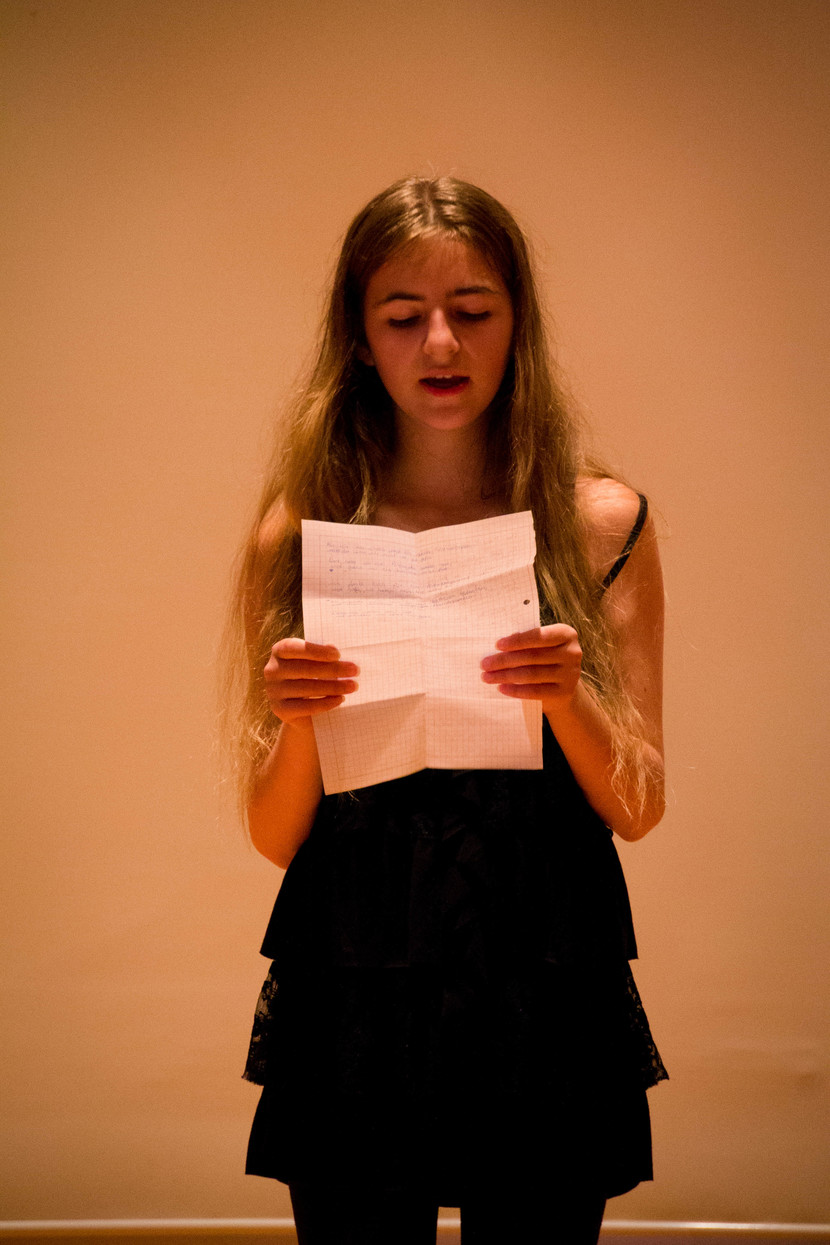
\includegraphics[width=0.6\textwidth]{impressionen/klein-11}%
    \hspace*{1cm}%
    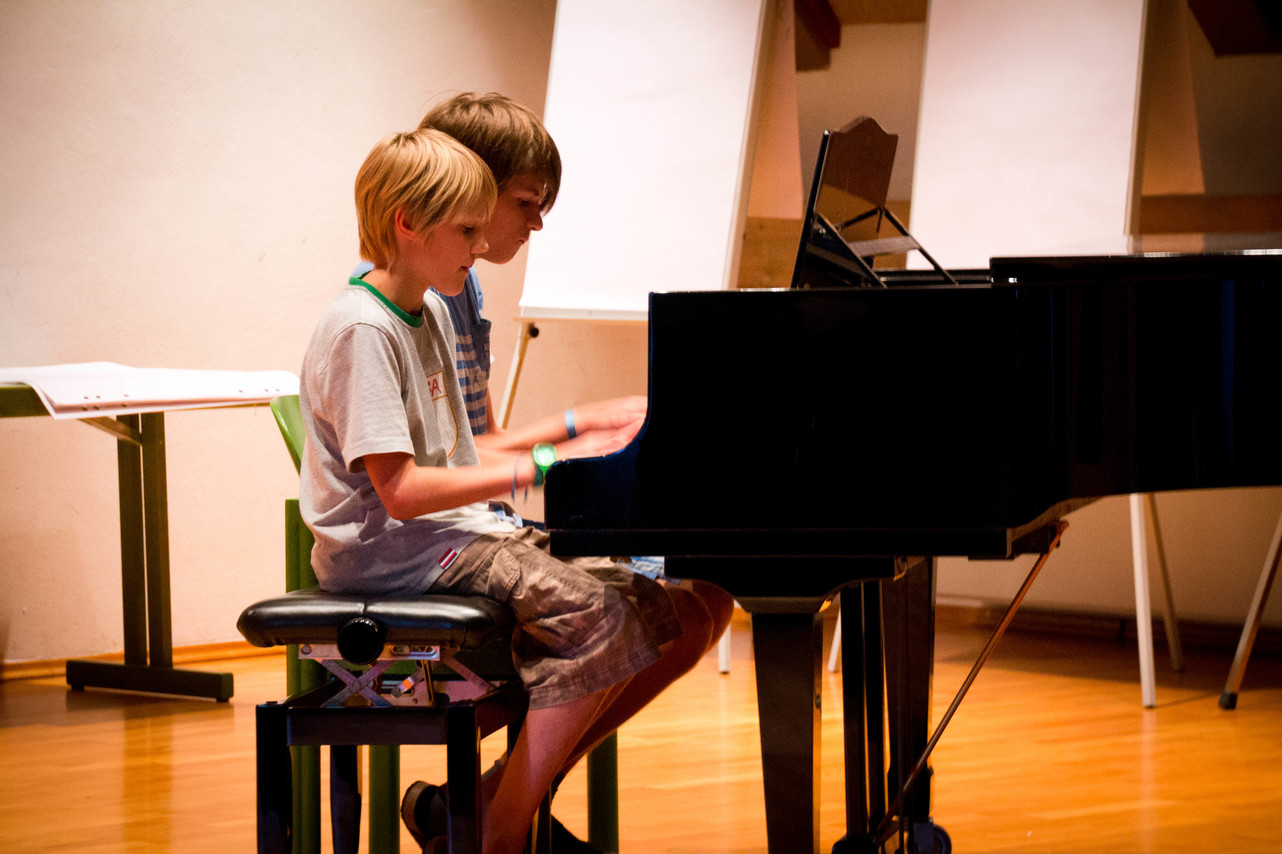
\includegraphics[width=0.6\textwidth]{impressionen/klein-12}%
  }

  \vfill

  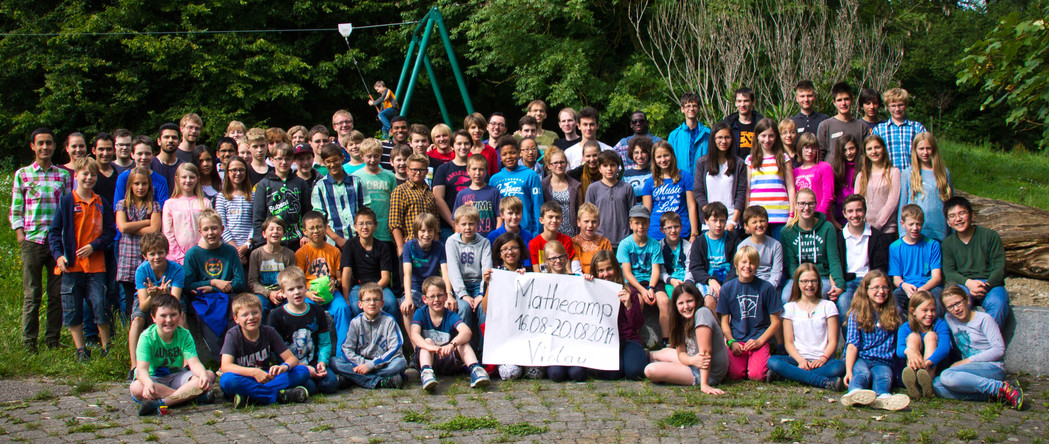
\includegraphics[width=\textwidth]{impressionen/klein-13}
\end{center}

\end{document}
